\chapter{Métodos e curvas de titulação}\label{ch:b1:titration-methods}

Uma farmacêutica recebe um lote de comprimidos de vitamina C rotulados
com \qty{500}{mg} e precisa certificar, antes da venda, que cada um
contém o que diz o rótulo. Ela não vai pesar a vitamina diretamente: ela
está misturada com aglutinantes e excipientes. Ela vai titulá-la ---
fazê-la reagir com um reagente de concentração conhecida, medir o volume
necessário e calcular a quantidade. Que reação usar, como ver o seu fim
e quão seguro é o resultado: essas são as perguntas deste capítulo, que
leva os equilíbrios dos cinco últimos capítulos para a bancada do
laboratório.

\begin{recall}
O volume escolar (anos 11 e 12) titulou ácidos com bases usando uma
mudança de cor, acompanhou \omterm{def:b1:titration-methods:titration}{titulações} com um pHmetro e um
condutivímetro e usou a relação de \omterm{def:b1:titration-methods:titration}{equivalência} $C_AV_A = C_BV_B$. O
método da \omterm{def:b1:predominant-reaction:predominant-reaction}{reação predominante} está no \cref{ch:b1:predominant-reaction};
os equilíbrios de precipitação, de complexação e de oxirredução, nos
\cref{ch:b1:precipitation,ch:b1:complexation,ch:b1:nernst}.
\end{recall}

\begin{omfigure}
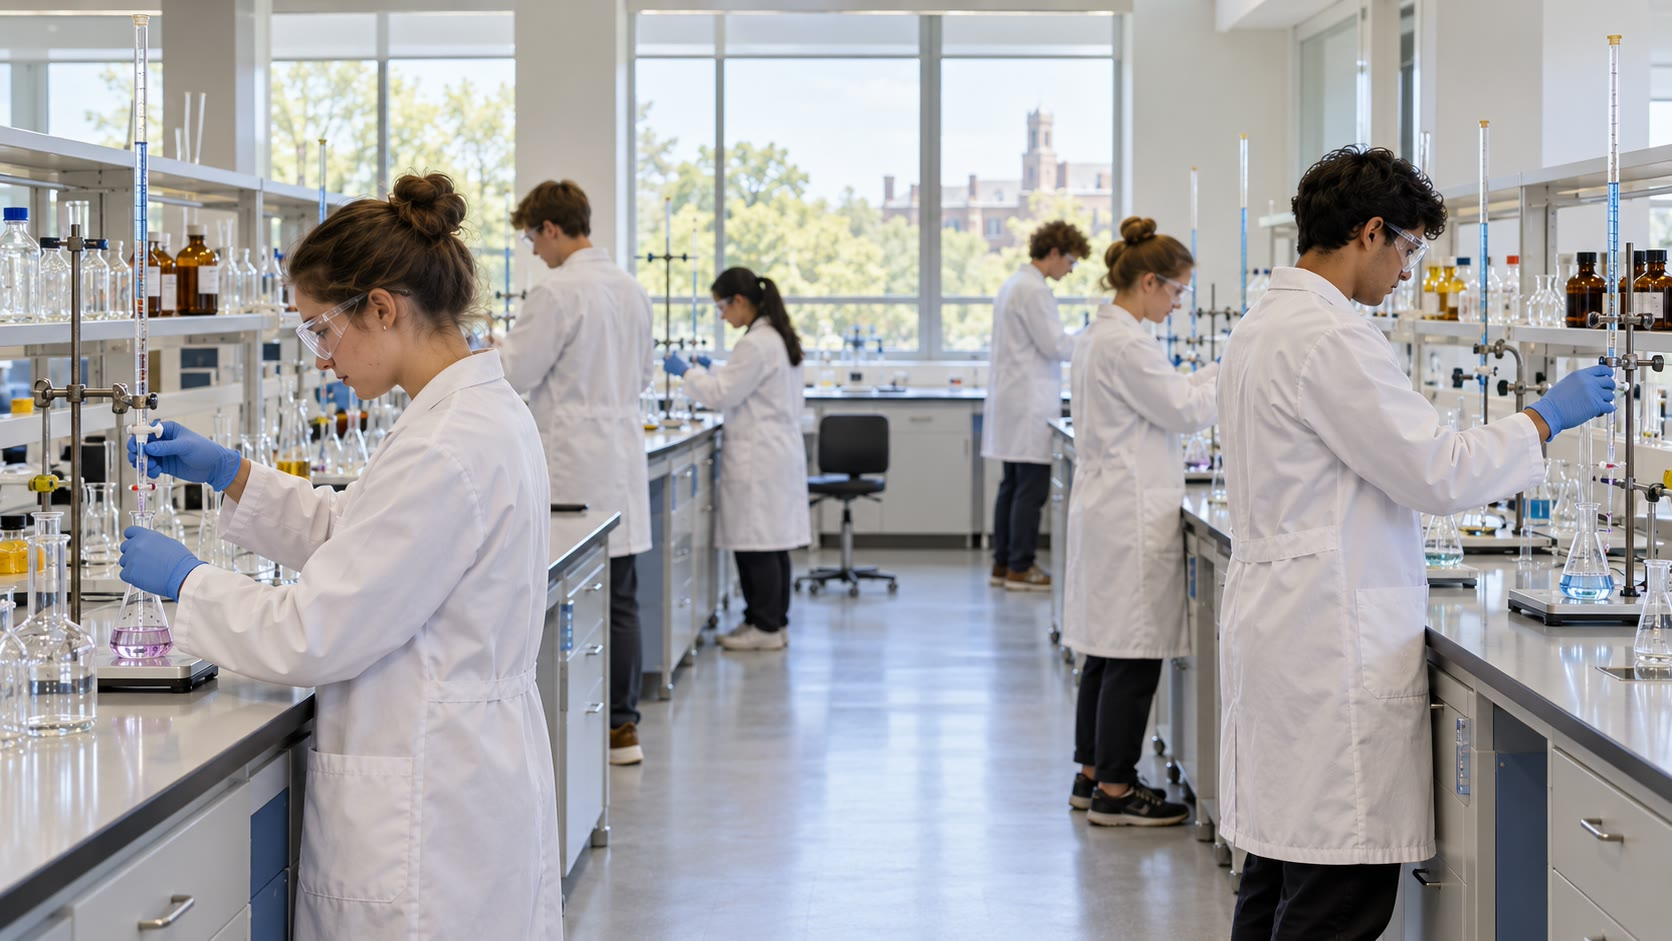
\includegraphics[width=0.66\linewidth]{images/book2/ai/b1-15-teaching-lab.jpg}

{\small Um laboratório de ensino: uma bureta, um erlenmeyer sobre um
agitador magnético, luvas e óculos. A \omterm{def:b1:titration-methods:titration}{titulação} é a medida quantitativa
mais comum em química.}
\end{omfigure}

\section{Titulação e equivalência}

\begin{definition}[Titulação, equivalência]\label{def:b1:titration-methods:titration}
Uma \emph{titulação}\index{titulacao@titulação} determina a quantidade de uma espécie,
o \emph{analito}\index{analito}, por meio de uma reação com um reagente
de concentração conhecida, o \emph{titulante}\index{titulante},
adicionado progressivamente. A reação deve ser única, \omterm{def:b1:extent-q-and-k:quantitative}{quantitativa} ($K$
grande) e rápida. A \emph{equivalência}\index{equivalencia@equivalência} é atingida
quando titulante e analito foram postos em contato nas proporções
estequiométricas da reação; o volume adicionado nesse momento é o
volume de equivalência, e o ponto da curva de titulação nesse volume é
o \emph{ponto de equivalência}\index{ponto de equivalencia@ponto de equivalência}. O volume em
que o experimentador para, ao ver uma mudança de cor ou uma quebra em
uma curva, é o \emph{ponto final}\index{ponto final}; um bom método faz
com que ele coincida com a equivalência.
\end{definition}

\begin{proposition}[Relação de equivalência]\label{prop:b1:titration-methods:equivalence}
Para uma reação de \omterm{def:b1:titration-methods:titration}{titulação} $a\,\mathrm{A} + b\,\mathrm{B} \to \cdots$,
com o \omterm{def:b1:titration-methods:titration}{analito} A ($n_A$ mol) e o \omterm{def:b1:titration-methods:titration}{titulante} B na concentração $C_B$, o
volume de \omterm{def:b1:titration-methods:titration}{equivalência} satisfaz
\[
  \frac{n_A}{a} = \frac{C_B V_{\mathrm{eq}}}{b} .
\]
\end{proposition}

\begin{proof}
Seja $x$ o avanço após a adição de um volume $V$ de \omterm{def:b1:titration-methods:titration}{titulante}. Antes da
\omterm{def:b1:titration-methods:titration}{equivalência}, B é o limitante e, sendo a \omterm{def:b1:extent-q-and-k:quantitative}{reação quantitativa},
$x = C_BV/b$; depois dela, A é o limitante e $x = n_A/a$. A \omterm{def:b1:titration-methods:titration}{equivalência}
é o volume em que os dois se esgotam juntos, $n_A - ax = 0$ e
$C_BV - bx = 0$: eliminar $x$ dá a relação.
\end{proof}

\section{Titulações diretas e indiretas}

\begin{definition}[Tipos de titulação]\label{def:b1:titration-methods:kinds}
Em uma \emph{titulação direta}\index{titulacao direta@titulação direta}, o \omterm{def:b1:titration-methods:titration}{titulante} reage
com o próprio \omterm{def:b1:titration-methods:titration}{analito}. Em uma \emph{titulação de retorno}\index{titulacao de retorno@titulação de retorno},
adiciona-se ao \omterm{def:b1:titration-methods:titration}{analito} um excesso conhecido de um reagente, e titula-se
o excesso que resta. Quando uma solução contém vários \omterm{def:b1:titration-methods:titration}{analitos} que
reagem um após o outro com o \omterm{def:b1:titration-methods:titration}{titulante}, eles são medidos por
\emph{titulações sucessivas}\index{titulacoes sucessivas@titulações sucessivas}, uma \omterm{def:b1:titration-methods:titration}{equivalência}
depois da outra; quando reagem juntos e dão uma única \omterm{def:b1:titration-methods:titration}{equivalência},
por uma \emph{titulação simultânea}\index{titulacao simultanea@titulação simultânea}, que só dá
a sua soma.
\end{definition}

\begin{method}[Titulação de retorno]\label{met:b1:titration-methods:back-titration}
Use-a quando a reação direta é lenta, quando o \omterm{def:b1:titration-methods:titration}{analito} é instável ou
volátil, ou quando nenhum indicador convém à reação direta.
\begin{enumerate}
  \item Adicione uma quantidade conhecida $n_R$ de reagente R, em
        excesso, e deixe-o reagir completamente com o \omterm{def:b1:titration-methods:titration}{analito} A
        ($\alpha\,\mathrm{A} + \rho\,\mathrm{R}$).
  \item Titule o excesso de R com um \omterm{def:b1:titration-methods:titration}{titulante} T ($\rho'\,\mathrm{R} +
        \tau\,\mathrm{T}$) até o volume de \omterm{def:b1:titration-methods:titration}{equivalência} $V_T$.
  \item Calcule $n_{R,\text{exc}} = \frac{\rho'}{\tau}C_TV_T$ e depois
        $n_A = \frac{\alpha}{\rho}(n_R - n_{R,\text{exc}})$.
\end{enumerate}
\end{method}

O problema de fim de semana titula a vitamina C dessa maneira: o ácido
ascórbico reduz um excesso de iodo, e o iodo restante é titulado pelo
tiossulfato.

\section{Titulações pHmétricas e indicadores}

\begin{omfigure}
\begin{tikzpicture}[font=\small]
  \pic at (0,0) {stirrer};
  \pic at (0,0.18) {beaker={0.55}{omDef!14}};
  \pic at (0.2,2.45) {burette={0.75}{white}};
  \pic at (-0.45,0.45) {probe};
  \pic (m) at (-2.6,3.2) {meter={pH}};
  \draw[thick] (-0.45,3.45) to[out=90, in=0] (m-b);
  \node[anchor=west] at (0.65,6.2) {bureta: NaOH, \qty{0.100}{mol/L}};
  \node[anchor=west] at (1.0,1.0) {ácido, $V_0 = \qty{10.0}{mL}$, diluído};
  \draw[<-, omProp, thick] (1.2,-0.25) -- (1.8,-0.25) node[anchor=west, text=black] {agitador magnético};
  \draw[<-, omProp, thick] (-0.62,2.4) -- (-1.5,2.0) node[anchor=east, text=black] {eletrodo combinado};
\end{tikzpicture}

{\small Uma \omterm{def:b1:titration-methods:titration}{titulação} pHmétrica. O eletrodo de vidro combinado mede o pH
após cada adição da bureta; o agitador mistura a solução. O eletrodo é
calibrado antes com duas \omterm{def:b1:predominant-reaction:buffer}{soluções-tampão}.}
\end{omfigure}

\begin{omfigure}
\begin{tikzpicture}
\begin{axis}[name=s,
  width=0.5\linewidth, height=5.6cm, xmin=0, xmax=20, ymin=0, ymax=14,
  axis x line=bottom, axis y line=left, xlabel={$V$ (mL)}, ylabel={pH},
  xtick={0,5,10,15,20}, ytick={0,2,4,6,8,10,12,14},
  tick label style={font=\small}, label style={font=\small}]
\addplot[omDef, very thick] table[x=V, y=pH] {figdata/out/bachelor-1-titration-curves-strong.dat};
\addplot[omProp, thick] table[x=V, y=pH] {figdata/out/bachelor-1-titration-curves-weak.dat};
\node[font=\scriptsize, omDef, anchor=south west] at (axis cs:6,0.2) {\ce{HCl}};
\node[font=\scriptsize, omProp, anchor=west] at (axis cs:0.4,6.4) {\ce{CH3COOH}};
\draw[dotted] (axis cs:5,0) -- (axis cs:5,4.76) -- (axis cs:0,4.76);
\node[font=\scriptsize, anchor=north] at (axis cs:2.5,4.7) {$\mathrm{p}K_a$};
\end{axis}
\begin{axis}[at={(s.east)}, anchor=west, xshift=1.2cm,
  width=0.5\linewidth, height=5.6cm, xmin=0, xmax=20, ymin=0, ymax=14,
  axis x line=bottom, axis y line=left, xlabel={$V$ (mL)}, ylabel={pH},
  xtick={0,5,10,15,20}, ytick={0,2,4,6,8,10,12,14},
  tick label style={font=\small}, label style={font=\small}]
\addplot[omMeth, very thick] table[x=V, y=pH] {figdata/out/bachelor-1-titration-curves-mixture.dat};
\node[font=\scriptsize, anchor=west, align=left] at (axis cs:10.8,6.0) {\ce{HCl} + \ce{CH3COOH}\\ duas equivalências};
\end{axis}
\end{tikzpicture}

{\small À esquerda: \qty{10.0}{mL} de ácido clorídrico e de ácido
etanoico, ambos a \qty{0.100}{mol/L}, titulados por hidróxido de sódio a
\qty{0.100}{mol/L}. O \omterm{def:b1:predominant-reaction:strong-acid}{ácido fraco} tem uma região tampão com pH $=
\mathrm{p}K_a$ na semiequivalência e um \omterm{def:b1:titration-methods:titration}{ponto de equivalência} em pH 8.73.
À direita: uma mistura, \qty{0.050}{mol/L} de cada ácido: o \omterm{def:b1:predominant-reaction:strong-acid}{ácido forte}
é titulado primeiro (\omterm{def:b1:titration-methods:titration}{equivalência} em \qty{5}{mL}), depois o fraco
(\qty{10}{mL}).}
\end{omfigure}

\begin{proposition}[Semiequivalência de um ácido fraco]\label{prop:b1:titration-methods:half-equivalence}
Quando um \omterm{def:b1:predominant-reaction:strong-acid}{ácido fraco} HA é titulado por uma \omterm{def:b1:predominant-reaction:strong-acid}{base forte}, na
semiequivalência $\mathrm{pH} = \mathrm{p}K_a$, desde que o ácido não
seja forte demais nem diluído demais ($\mathrm{p}K_a$ aproximadamente
entre 4 e 10 a
\qty{0.1}{mol/L}).
\end{proposition}

\begin{proof}
Na semiequivalência, a \omterm{def:b1:extent-q-and-k:quantitative}{reação quantitativa} \ce{HA + OH- -> A- + H2O}
converteu metade de HA: $[\mathrm{HA}] = [\mathrm{A^-}]$, e a relação de
Henderson dá $\mathrm{pH} = \mathrm{p}K_a$. A condição garante que a
reação de HA com a água e a de $\mathrm{A^-}$ com a água não alteram
apreciavelmente essas quantidades.
\end{proof}

\begin{proposition}[pH na equivalência de um ácido fraco]\label{prop:b1:titration-methods:ph-at-equivalence}
Na \omterm{def:b1:titration-methods:titration}{equivalência} de um \omterm{def:b1:predominant-reaction:strong-acid}{ácido fraco} ($\mathrm{p}K_a$) por uma \omterm{def:b1:predominant-reaction:strong-acid}{base forte}, a
solução é a base conjugada na concentração $C'$ (após diluição), e
\[
  \mathrm{pH} = \tfrac12(\mathrm{p}K_e + \mathrm{p}K_a + \log C') .
\]
\end{proposition}

\begin{proof}
A \omterm{def:b1:predominant-reaction:predominant-reaction}{reação predominante} da base com a água,
\ce{A- + H2O <=> HA + OH-}, tem $K = K_e/K_a$; com pouca base
convertida, $[\ce{OH-}] = \sqrt{KC'}$ (\cref{prop:b1:predominant-reaction:ph-formulas}),
donde o resultado. Para o ácido etanoico, $C' = \qty{0.050}{mol/L}$:
$\frac12(14.00 + 4.76 - 1.30) = 8.73$.
\end{proof}

\begin{proposition}[Titulações sucessivas]\label{prop:b1:titration-methods:successive}
Dois ácidos titulados pela mesma base dão \omterm{def:b1:titration-methods:titration}{equivalências} separadas, cada
uma com precisão melhor que \qty{1}{\percent}, se seus $\mathrm{p}K_a$
diferirem de pelo menos 4.
\end{proposition}

\begin{proof}
Na primeira \omterm{def:b1:titration-methods:titration}{equivalência}, a reação da base $\mathrm{A_1^-}$ com o
segundo ácido $\mathrm{HA_2}$, $\mathrm{A_1^-} + \mathrm{HA_2}
\rightleftharpoons \mathrm{HA_1} + \mathrm{A_2^-}$, tem $K = 10^{\mathrm{p}K_1 - \mathrm{p}K_2}$.
Partindo de quantidades iguais, a fração $x$ do segundo ácido já
titulada satisfaz $x^2/(1 - x)^2 = K$; para $x \leqslant 0.01$, $K
\leqslant 10^{-4}$, isto é, $\mathrm{p}K_2 - \mathrm{p}K_1 \geqslant 4$.
\end{proof}

O ácido fosfórico (2.15, 7.21, 12.34) dá duas \omterm{def:b1:titration-methods:titration}{equivalências} nítidas; a
terceira se perde na água da base. O ácido etanoico misturado ao ácido
clorídrico (à direita da figura) é titulado depois dele, sendo o \omterm{def:b1:predominant-reaction:strong-acid}{ácido
forte}, na prática, um $\mathrm{p}K_a$ abaixo de 0.

\begin{method}[Localizar uma equivalência em uma curva]\label{met:b1:titration-methods:derivative}
\begin{enumerate}
  \item Derivada: calcule $\Delta\mathrm{pH}/\Delta V$ entre pontos
        sucessivos; a \omterm{def:b1:titration-methods:titration}{equivalência} fica em seu máximo.
  \item Tangentes: trace duas tangentes paralelas à curva de cada lado do
        salto, e a paralela equidistante delas; ela corta a curva no \omterm{def:b1:titration-methods:titration}{ponto
        de equivalência}.
\end{enumerate}
\end{method}

\begin{method}[Tangentes, por cálculo]\label{met:b1:titration-methods:tangents}
Para uma curva registrada por computador, ajuste os pontos de cada lado
do salto por uma função suave e tome o ponto de inflexão; para um salto
simétrico (\omterm{def:b1:predominant-reaction:strong-acid}{ácido forte}, \omterm{def:b1:predominant-reaction:strong-acid}{base forte}), o meio do salto em pH 7 é o \omterm{def:b1:titration-methods:titration}{ponto
de equivalência}.
\end{method}

\begin{definition}[Indicador colorido, faixa de viragem]\label{def:b1:titration-methods:indicator}
Um \emph{indicador colorido}\index{indicador colorido} é um \omterm{def:b1:predominant-reaction:bronsted}{par ácido--base} fraco
HIn/In$^-$ cujas duas formas têm cores diferentes. Sua cor muda ao longo
da \emph{faixa de viragem}\index{faixa de viragem}, o intervalo de pH em que
nenhuma das formas predomina claramente, cerca de
$\mathrm{p}K_{a}(\mathrm{HIn}) \pm 1$.
\end{definition}

\begin{omfigure}
\begin{tabular}{lccl}
\hline
indicador & $\mathrm{p}K_a$ & \omterm{def:b1:titration-methods:indicator}{faixa de viragem} & cores (ácida / básica) \\
\hline
alaranjado de metila & 3.5 & 2.5--4.5 & vermelho / amarelo \\
vermelho de metila & 4.8 & 3.8--5.8 & vermelho / amarelo \\
vermelho de fenol & 7.9 & 6.9--8.9 & amarelo / vermelho \\
azul de timol (segunda viragem) & 9.2 & 8.2--10.2 & amarelo / azul \\
\hline
\end{tabular}

\smallskip
{\small Quatro indicadores, $\mathrm{p}K_a$ tirados de uma compilação
crítica de \omterm{def:b1:complexation:formation-constant}{constantes de dissociação}; as \omterm{def:b1:titration-methods:indicator}{faixas de viragem} são
$\mathrm{p}K_a \pm 1$.}
% ledger: pka:methylorange, pka:methylred, pka:phenolred, pka:thymolblue2
\end{omfigure}

\begin{method}[Escolher um indicador]\label{met:b1:titration-methods:choose-indicator}
Escolha um indicador cuja \omterm{def:b1:titration-methods:indicator}{faixa de viragem} fique dentro do salto vertical
da curva, o mais perto possível do pH na \omterm{def:b1:titration-methods:titration}{equivalência}. \omterm{def:b1:predominant-reaction:strong-acid}{Ácido forte} por
\omterm{def:b1:predominant-reaction:strong-acid}{base forte} (salto de 3.3 a 10.7 para $\pm\qty{0.1}{mL}$ aqui): qualquer
um dos quatro. Ácido etanoico (\omterm{def:b1:titration-methods:titration}{equivalência} em 8.73): vermelho de fenol
ou azul de timol; o alaranjado de metila mudaria de cor muito antes da
\omterm{def:b1:titration-methods:titration}{equivalência}.
\end{method}

\section{Titulações potenciométricas}

\begin{definition}[Titulação potenciométrica]\label{def:b1:titration-methods:potentiometric}
Uma \emph{titulação potenciométrica}\index{titulacao potenciometrica@titulação potenciométrica}
acompanha o potencial de um eletrodo na solução em relação a um \omterm{def:b1:nernst:reference-electrode}{eletrodo
de referência}, para uma \omterm{def:b1:titration-methods:titration}{titulação} de oxirredução (fio de platina), de
precipitação (fio de prata) ou de complexação.
\end{definition}

\begin{proposition}[Pontos notáveis de uma titulação de oxirredução]\label{prop:b1:titration-methods:potentiometric-points}
Para a \omterm{def:b1:titration-methods:titration}{titulação} de $\mathrm{Red_1}$ por $\mathrm{Ox_2}$ com
$n_2\,\mathrm{Red_1} + n_1\,\mathrm{Ox_2} \to n_2\,\mathrm{Ox_1} +
n_1\,\mathrm{Red_2}$ (pares de $n_1$ e $n_2$ elétrons), $E(V_{\mathrm{eq}}/2) = E^\circ_1$, $E(2V_{\mathrm{eq}}) =
E^\circ_2$, e na \omterm{def:b1:titration-methods:titration}{equivalência}
\[
  E_{\mathrm{eq}} = \frac{n_1E^\circ_1 + n_2E^\circ_2}{n_1 + n_2},
\]
para pares cujas \omterm{def:b1:nernst:couple}{semirreações} não envolvem outras espécies (ou em um pH
que mantém fixos os termos adicionais).
\end{proposition}

\begin{proof}
Na semiequivalência, metade de $\mathrm{Red_1}$ está oxidada:
$[\mathrm{Ox_1}] = [\mathrm{Red_1}]$ e a \omterm{thm:b1:nernst:nernst}{equação de Nernst} do par 1 dá
$E^\circ_1$. Em $2V_{\mathrm{eq}}$, há tanto $\mathrm{Ox_2}$ em excesso
quanto foi reduzido: $[\mathrm{Ox_2}] = [\mathrm{Red_2}]$, $E = E^\circ_2$.
Na \omterm{def:b1:titration-methods:titration}{equivalência}, multiplique a \omterm{thm:b1:nernst:nernst}{equação de Nernst} do par 1 por $n_1$ e a
do par 2 por $n_2$ e some; a estequiometria faz com que
$[\mathrm{Ox_1}]/[\mathrm{Red_1}] \cdot [\mathrm{Ox_2}]/[\mathrm{Red_2}] = 1$
(as quantidades de $\mathrm{Red_1}$ e de $\mathrm{Ox_2}$ restantes estão
na mesma proporção que os produtos), de modo que os logaritmos se
cancelam.
\end{proof}

Para o ferro(II) pelo permanganato em ácido a \qty{1}{mol/L}, $n_1 = 1$ e
$n_2 =
5$: $E_{\mathrm{eq}} = (0.77 + 5 \times 1.51)/6 = 1.39$~V. O salto,
de cerca de 0.8 a 1.5~V, é tão grande que o \omterm{def:b1:titration-methods:titration}{ponto final} é nítido; na
prática, o permanganato é o seu próprio indicador, com sua cor violeta
persistindo na primeira gota em excesso.

\begin{omfigure}
\begin{tikzpicture}
\begin{axis}[name=p,
  width=0.5\linewidth, height=5.6cm, xmin=0, xmax=20, ymin=0.6, ymax=1.6,
  axis x line=bottom, axis y line=left, xlabel={$V$ (mL)}, ylabel={$E$ (V)},
  xtick={0,5,10,15,20},
  tick label style={font=\small}, label style={font=\small}]
\addplot[omDef, very thick] table[x=V, y=E] {figdata/out/bachelor-1-titration-curves-potentiometric.dat};
\draw[dotted] (axis cs:5,0.6) -- (axis cs:5,0.77) -- (axis cs:0,0.77);
\draw[dotted] (axis cs:10,0.6) -- (axis cs:10,1.39) -- (axis cs:0,1.39);
\node[font=\scriptsize, anchor=south west] at (axis cs:0.2,0.77) {0.77};
\node[font=\scriptsize, anchor=south west] at (axis cs:0.2,1.39) {1.39};
\end{axis}
\begin{axis}[at={(p.east)}, anchor=west, xshift=1.2cm,
  width=0.5\linewidth, height=5.6cm, xmin=0, xmax=20, ymin=0, ymax=4.6,
  axis x line=bottom, axis y line=left, xlabel={$V$ (mL)},
  ylabel={$\kappa$ (mS/cm)}, xtick={0,5,10,15,20},
  tick label style={font=\small}, label style={font=\small}]
\addplot[omProp, very thick] table[x=V, y=kappa] {figdata/out/bachelor-1-titration-curves-conductimetric.dat};
\draw[dotted] (axis cs:10,0) -- (axis cs:10,1.15);
\end{axis}
\end{tikzpicture}

{\small À esquerda: \omterm{def:b1:titration-methods:potentiometric}{titulação potenciométrica} de \qty{10.0}{mL} de
ferro(II) a \qty{0.100}{mol/L} pelo permanganato a \qty{0.0200}{mol/L}
em ácido a \qty{1}{mol/L} (eletrodo de platina, potencial em relação ao
eletrodo de hidrogênio). À direita: \omterm{def:b1:titration-methods:titration}{titulação} condutométrica de
\qty{100}{mL} de ácido clorídrico a \qty{0.0100}{mol/L} por hidróxido de
sódio a \qty{0.100}{mol/L}; a \omterm{def:b1:titration-methods:titration}{equivalência} fica na interseção de duas
retas.}
% ledger: lam:H+, lam:OH-, lamsalt:HCl, lamsalt:NaCl (conductivities in figdata/bachelor-1/titration-curves.py)
\end{omfigure}

\section{Titulações condutométricas, complexométricas e por precipitação}

\begin{definition}[Condutividade molar iônica]\label{def:b1:titration-methods:conductivity}
A condutividade $\kappa$ de uma solução (em \unit{S/m}) mede a
facilidade com que ela conduz corrente pelo movimento de seus íons. A
\emph{condutividade molar iônica}\index{condutividade molar ionica@condutividade molar iônica}
$\lambda_i$ de um íon é a sua contribuição por mol por unidade de
volume; seu valor em diluição infinita, $\lambda_i^\circ$, é uma
constante do íon e do solvente a uma dada temperatura.
\end{definition}

\begin{proposition}[Lei de Kohlrausch]\label{prop:b1:titration-methods:kohlrausch}
Em solução diluída, a condutividade é a soma das contribuições dos
íons,
\[
  \kappa = \sum_i \lambda_i^\circ c_i ,
\]
a \emph{lei de Kohlrausch}\index{lei de Kohlrausch}; a condutividade molar de
um sal é a soma das de seus íons.
\end{proposition}

\admitted{A \omterm{prop:b1:titration-methods:kohlrausch}{lei de Kohlrausch} exprime que os íons diluídos se movem
independentemente; seus limites em concentrações mais altas são
estudados no volume do 2.º~ano. Aqui, ela é usada como lei
experimental.}

\begin{proposition}[Inclinações de uma titulação condutométrica]\label{prop:b1:titration-methods:conductimetric-slopes}
Quando um \omterm{def:b1:predominant-reaction:strong-acid}{ácido forte} H$^+$X$^-$ é titulado por uma \omterm{def:b1:predominant-reaction:strong-acid}{base forte}
Na$^+$OH$^-$ em um grande volume (diluição desprezada), a condutividade
varia linearmente com o volume adicionado, com inclinação proporcional a
$\lambda^\circ(\ce{Na+}) - \lambda^\circ(\ce{H+}) < 0$ antes da
\omterm{def:b1:titration-methods:titration}{equivalência} e a $\lambda^\circ(\ce{Na+}) + \lambda^\circ(\ce{OH-}) > 0$
depois.
\end{proposition}

\begin{proof}
Antes da \omterm{def:b1:titration-methods:titration}{equivalência}, cada mol de hidróxido adicionado retira um mol de
\ce{H+} (\ce{H+ + OH- -> H2O}) e traz um mol de \ce{Na+}; depois da
\omterm{def:b1:titration-methods:titration}{equivalência}, ele acrescenta um \ce{Na+} e um \ce{OH-}. \ce{X-} não
muda. Pela \omterm{prop:b1:titration-methods:kohlrausch}{lei de Kohlrausch}, a condutividade varia dessas combinações de
$\lambda^\circ$ vezes a quantidade adicionada dividida pelo volume (fixo).
\end{proof}

A partir das condutividades limite, $\lambda^\circ(\ce{H+}) =
\qty{349.8}{S.cm^2/mol}$ e $\lambda^\circ(\ce{OH-}) = 198.3$, e das dos
sais \ce{HCl} (426) e \ce{NaCl} (126.5), a \omterm{prop:b1:titration-methods:kohlrausch}{lei de Kohlrausch} dá
$\lambda^\circ(\ce{Cl-}) = 426 - 349.8 = 76.2$ e $\lambda^\circ(\ce{Na+}) =
126.5 - 76.2 = 50.3$~\unit{S.cm^2/mol}. Os íons hidrogênio e hidróxido
conduzem muito melhor que os outros: a curva é um V bem marcado.

As \omterm{def:b1:titration-methods:titration}{titulações} complexométricas usam o edta: em pH 10 (tampão amoniacal),
o cálcio e o magnésio reagem com ele quantitativamente (constantes
condicionais do \cref{ch:b1:complexation}), e um indicador que é ele
próprio um complexante fraco do metal muda de cor quando o edta lhe
retira os últimos íons metálicos --- a \omterm{def:b1:titration-methods:titration}{titulação} da dureza da água. As
\omterm{def:b1:titration-methods:titration}{titulações} por precipitação usam os íons prata: o cloreto é titulado
pelo nitrato de prata com o cromato como indicador
(\cref{exo:b1:precipitation:8}), ou acompanhado com um eletrodo de prata
(\cref{ch:b1:nernst}). A precisão de todos esses resultados, fixada pela
vidraria e pelo \omterm{def:b1:titration-methods:titration}{ponto final}, é tratada no
\cref{ch:b1:lab-techniques-1}.

\section{Exercícios}

\begin{exercise}[$\star$]\label{exo:b1:titration-methods:1}
\qty{20.0}{mL} de uma solução de hidróxido de sódio precisam de
\qty{12.4}{mL} de ácido clorídrico a \qty{0.100}{mol/L}. Escreva a
reação, sua constante, e calcule a concentração da base.
\end{exercise}

\begin{exercise}[$\star$]\label{exo:b1:titration-methods:2}
Que indicador da tabela convém à \omterm{def:b1:titration-methods:titration}{titulação} da amônia (\qty{0.10}{mol/L},
$\mathrm{p}K_a = 9.25$) pelo ácido clorídrico a \qty{0.10}{mol/L}? Calcule
antes o pH na \omterm{def:b1:titration-methods:titration}{equivalência}.
\end{exercise}

\begin{exercise}[$\star$]\label{exo:b1:titration-methods:3}
\qty{10.0}{mL} de ferro(II) são titulados pelo permanganato a
\qty{0.0200}{mol/L}; a cor violeta persiste a partir de \qty{12.6}{mL}.
Escreva a reação e calcule a concentração de ferro(II).
\end{exercise}

\begin{exercise}[$\star$]\label{exo:b1:titration-methods:4}
Uma amostra de água de \qty{50.0}{mL} é titulada pelo edta a
\qty{0.0100}{mol/L} em pH 10; a \omterm{def:b1:titration-methods:titration}{equivalência} fica em \qty{14.2}{mL}. O
edta reage um para um com o cálcio e o magnésio. Calcule a concentração
total desses dois íons. Trata-se de uma \omterm{def:b1:titration-methods:kinds}{titulação simultânea} ou
sucessiva?
\end{exercise}

\begin{exercise}[$\star\star$]\label{exo:b1:titration-methods:5}
Para a \omterm{def:b1:titration-methods:titration}{titulação} de \qty{10.0}{mL} de ácido etanoico a \qty{0.100}{mol/L}
por hidróxido de sódio a \qty{0.100}{mol/L}, calcule o pH em 0, 5.0, 10.0
e \qty{15.0}{mL} com os métodos do \cref{ch:b1:predominant-reaction}, e
compare com a curva deste capítulo.
\end{exercise}

\begin{exercise}[$\star\star$]\label{exo:b1:titration-methods:6}
Mostre que uma \omterm{def:b1:titration-methods:titration}{titulação} pHmétrica do ácido fosfórico por hidróxido de
sódio dá dois saltos, e calcule o pH em cada \omterm{def:b1:titration-methods:titration}{equivalência} para um ácido
a \qty{0.100}{mol/L} (\qty{10.0}{mL}, base a \qty{0.100}{mol/L}). Por que
não há um terceiro salto?
\end{exercise}

\begin{exercise}[$\star\star$]\label{exo:b1:titration-methods:7}
Uma mistura de ácido clorídrico e ácido etanoico (\qty{10.0}{mL}) é
titulada por hidróxido de sódio a \qty{0.100}{mol/L}: duas \omterm{def:b1:titration-methods:titration}{equivalências},
em \qty{6.2}{mL} e \qty{14.6}{mL}. Calcule as duas concentrações. Qual é
o pH a meio caminho entre as duas \omterm{def:b1:titration-methods:titration}{equivalências}?
\end{exercise}

\begin{exercise}[$\star\star$]\label{exo:b1:titration-methods:8}
Calcule o potencial do eletrodo de platina na \omterm{def:b1:titration-methods:titration}{titulação} do ferro(II) pelo
permanganato (dados do capítulo) em 2.0, 9.0, 11.0 e \qty{20.0}{mL}.
\end{exercise}

\begin{exercise}[$\star\star$]\label{exo:b1:titration-methods:9}
Usando a \omterm{prop:b1:titration-methods:kohlrausch}{lei de Kohlrausch} e os valores do capítulo, calcule a
condutividade do ácido clorídrico titulado em 0, 10.0 e \qty{20.0}{mL} de
base (\qty{100}{mL} de ácido a \qty{0.0100}{mol/L}, base a
\qty{0.100}{mol/L}, levando em conta a diluição), e as duas inclinações.
\end{exercise}

\begin{exercise}[$\star\star\star$]\label{exo:b1:titration-methods:10}
Demonstre que a curva pHmétrica de um \omterm{def:b1:predominant-reaction:strong-acid}{ácido forte} titulado por uma \omterm{def:b1:predominant-reaction:strong-acid}{base
forte} é simétrica em relação ao \omterm{def:b1:titration-methods:titration}{ponto de equivalência} quando a diluição
é desprezada, e calcule a amplitude do salto entre
$V_{\mathrm{eq}} \pm 0.1$~mL para a \omterm{def:b1:titration-methods:titration}{titulação} do capítulo. Como ela muda
se todas as concentrações forem divididas por 100?
\end{exercise}

\begin{exercise}[$\star\star\star$]\label{exo:b1:titration-methods:11}
Deduza a equação da curva potenciométrica do ferro(II) pelo permanganato
antes e depois da \omterm{def:b1:titration-methods:titration}{equivalência}, e verifique os três pontos notáveis da
\cref{prop:b1:titration-methods:potentiometric-points}. Como mudaria o
potencial de \omterm{def:b1:titration-methods:titration}{equivalência} em pH 1?
\end{exercise}

\begin{exercise}[$\star\star\star$]\label{exo:b1:titration-methods:12}
O cloreto de amônio (\qty{0.100}{mol/L}, $\mathrm{p}K_a = 9.25$) não pode
ser titulado com exatidão por hidróxido de sódio com um indicador.
Explique a partir da curva e, depois, proponha uma \omterm{def:b1:titration-methods:kinds}{titulação de retorno}:
excesso de hidróxido de sódio, expulsão da amônia por fervura, \omterm{def:b1:titration-methods:titration}{titulação}
do hidróxido restante com ácido clorídrico. Escreva o cálculo.
\end{exercise}

\section{Problema: Quanta vitamina C há no comprimido?}

\begin{problem}[{Problema de fim de semana --- a reação do iodo com o ácido
ascórbico, uma titulação de retorno pelo tiossulfato, o cálculo do
resultado e sua incerteza, terminando na massa de ácido ascórbico por
comprimido}]
\label{pb:b1:titration-methods:1}
Um comprimido é triturado e dissolvido em água em um balão volumétrico de
\qty{100.0}{mL}. Retira-se uma alíquota de \qty{10.00}{mL} com uma
pipeta, e adicionam-se \qty{20.00}{mL} de solução de iodo a
\qty{0.0250}{mol/L} (excesso). O iodo restante é titulado pelo
tiossulfato de sódio a \qty{0.0500}{mol/L} com amido como indicador: a
cor azul desaparece em \qty{8.90}{mL}. O ácido ascórbico é \ce{C6H8O6}
($M = \qty{176.0}{g/mol}$); o iodo o oxida a \ce{C6H6O6}.
$E^\circ(\ce{I2}/\ce{I-}) = 0.53$~V,
$E^\circ(\ce{S4O6^2-}/\ce{S2O3^2-}) = 0.02$~V.

\medskip
\noindent\textbf{Parte I --- As reações.}
\begin{enumerate}
  \item Escreva a \omterm{def:b1:nernst:couple}{semirreação} do par \ce{C6H6O6}/\ce{C6H8O6}.
  \item Escreva a reação do iodo com o ácido ascórbico.
  \item Dê o \omterm{def:b1:nernst:oxidation-number}{número de oxidação} do iodo em \ce{I2} e em \ce{I-}.
  \item Escreva a reação do iodo com o tiossulfato e calcule sua
        constante.
  \item O amido dá uma cor azul intensa com o iodo. Por que a cor
        desaparece exatamente na \omterm{def:b1:titration-methods:titration}{equivalência} da \omterm{def:b1:titration-methods:titration}{titulação} pelo
        tiossulfato?
  \item O ácido ascórbico é lentamente oxidado pelo oxigênio do ar. Por
        que isso justifica adicionar o iodo de uma vez, em excesso?
\end{enumerate}

\medskip
\noindent\textbf{Parte II --- Por que uma \omterm{def:b1:titration-methods:kinds}{titulação de retorno}?}
\begin{enumerate}[resume]
  \item O que exigiria uma \omterm{def:b1:titration-methods:kinds}{titulação direta} do ácido ascórbico pelo iodo?
  \item Descreva a \omterm{def:b1:titration-methods:kinds}{titulação de retorno} como as três etapas do
        \cref{met:b1:titration-methods:back-titration}.
  \item Por que o iodo precisa estar em excesso? Verifique isso com o
        resultado.
  \item Por que a solução de tiossulfato é padronizada pouco antes do uso?
  \item A alíquota é de \qty{10.00}{mL} em \qty{100.0}{mL}: qual é o
        fator de diluição?
  \item Que vidraria fornece os \qty{20.00}{mL} de solução de iodo?
\end{enumerate}

\medskip
\noindent\textbf{Parte III --- O cálculo.}
\begin{enumerate}[resume]
  \item Calcule a quantidade de iodo introduzida.
  \item Calcule a quantidade de tiossulfato usada.
  \item Deduza a quantidade de iodo em excesso.
  \item Deduza a quantidade de iodo que reagiu com o ácido ascórbico.
  \item Calcule a quantidade de ácido ascórbico na alíquota.
  \item Calcule a quantidade e, depois, a massa de ácido ascórbico no
        comprimido.
  \item Compare com o rótulo (\qty{500}{mg}).
\end{enumerate}

\medskip
\noindent\textbf{Parte IV --- Quão seguro?}
As tolerâncias são: balão \qty{100.0 \pm 0.1}{mL}, pipetas
\qty{10.00 \pm 0.02}{mL} e \qty{20.00 \pm 0.03}{mL}, leitura da bureta
$\pm\qty{0.05}{mL}$; as duas concentrações são conhecidas a
\qty{0.2}{\percent}.
\begin{enumerate}[resume]
  \item Expresse $n(\text{ácido ascórbico})$ no comprimido em função das
        grandezas medidas.
  \item Que incertezas relativas entram na quantidade de iodo introduzida
        e na quantidade em excesso?
  \item Por que uma diferença de duas quantidades amplifica a incerteza
        relativa?
  \item Combinando as contribuições como no \cref{ch:b1:lab-techniques-1}
        (soma quadrática), estime a incerteza relativa do resultado.
  \item Dê a massa de ácido ascórbico por comprimido com sua incerteza,
        com dois algarismos significativos.
\end{enumerate}
\end{problem}
